\capitulo{5}{Aspectos relevantes del desarrollo del proyecto}

%Debe incluir desde la exposición del ciclo de vida utilizado, hasta los detalles de mayor relevancia de las fases de análisis, diseño e implementación.
%Se busca que no sea una mera operación de copiar y pegar diagramas y extractos del código fuente, sino que realmente se justifiquen los caminos de solución que se han tomado, especialmente aquellos que no sean triviales.
%Puede ser el lugar más adecuado para documentar los aspectos más interesantes del diseño y de la implementación, con un mayor hincapié en aspectos tales como el tipo de arquitectura elegido, los índices de las tablas de la base de datos, normalización y desnormalización, distribución en ficheros3, reglas de negocio dentro de las bases de datos (EDVHV GH GDWRV DFWLYDV), aspectos de desarrollo relacionados con el WWW...
%Este apartado, debe convertirse en el resumen de la experiencia práctica del proyecto, y por sí mismo justifica que la memoria se convierta en un documento útil, fuente de referencia para los autores, los tutores y futuros alumnos.

Este capítulo trata de recoger los aspectos más interesantes del desarrollo del proyecto. Las diferentes decisiones que se tomaron, pasando por los múltiples problemas que se sucedieron, propios de un proyecto creado desde cero y cómo se fueron solventando.

%\label{sec:ciclodevida}
\section{Ciclo de vida del desarrollo}       
El proyecto ha ido desarrollándose y se ha distribuido de forma semanal, basándonos en la metodología ágil Scrum. De forma que cada semana había una reunión con el tutor, en las que se veía el estado del proyecto y se establecían las nuevas tareas.

Lo primero fue instalar el entorno de desarrollo, una vez configurado y con el sistema embebido en mi poder, me puse manos a la obra y fui viendo cómo funcionaba la placa, el módulo gps y el IDE. Una vez hechas las conexiones del módulo gps, para que pudieran pasar los datos a la placa, se pudo ver por primera vez gracias a un pequeño código, cómo se mostraban los mensajes NMEA por pantalla, en la terminal de Termite. 
\imagen{conexiones.PNG}{Conexiones hechas entre los pines Rx y Tx hacia Digital I/O 1 y 0 respectivamente.}

El siguiente paso fue ver cómo funcionaba el acelerómetro que incorporaba la placa, para ello se decidió hacer un programa que almacenase los datos recogidos por él mismo en la tarjeta microSD. 

Para ello, se necesitaban crear y configurar diferentes módulos para que pudiesen funcionar, nos hemos basado en unos tutoriales que, a pesar de estar en algunos casos desactualizados, nos han servido de base \cite{tutorial}. Algunos de estos módulos fueron: 
\begin{itemize}
\tightlist
\item
	El sistema de almacenamiento.
\item
	El componente del acelerómetro.
\item
	El componente de la unidad de tiempo.	
\item
	El componente de la fecha.
\item
	El componente de secciones críticas.
\item
	El componente de la tarjeta microSD.
\item
	El componente de la comunicación síncrona.
\end{itemize}
Cabe destacar que la mayoría de estas interfaces necesitan una pequeña configuración en sus parámetros para que sean funcionales y se terminen de acoplar con el resto del sistema, no entraremos en detalle ya que considero que se escapa del objetivo de esta memoria, sin embargo queda citado por si fuera de interés\cite{tutorial}.
Finalmente, tras esto y una pequeña función, teníamos los datos del acelerómetro en la tarjeta microSD. 

Era el momento hacer lo mismo con los mensajes NMEA proporcionados por el módulo GPS, pero antes había que instalar dos módulos más\cite{tutorial2}, el de una interrupción externa y el de una señal asíncrona que sería la encargada de pasar los datos del módulo GPS a la placa. De esta forma ya podíamos almacenar las coordenadas en un archivo de texto.
\imagen{placa.PNG}{Placa de desarrollo FRDMK64F con el módulo GPS integrado y registrando datos.}

A continuación vendría la creación de la interfaz para poder mostrar las coordenadas, previamente almacenadas.
Se hizo una primera versión de una interfaz que simplemente mostrara un mapa donde poder representar coordenadas, para ello nos ayudamos de una API como es Mapbox. En este punto del proyecto se consiguió representar por primera vez una ruta. Sin embargo debía automatizar el proceso ya que la conversión de los datos arrojados por la placa (NMEA) y los leídos por la API de Mapbox había sido realizada de forma manual, mediante una herramienta de internet. 

El primer paso consistía en transformar los datos de NMEA a GeoJSON de forma automática, para ello, fue imprescindible la ayuda de la API de MyGeodata, realizando un script en Python que se encargaba de ello.
A partir de ahí vino la implementación de la subida de archivos al servidor, para así poder pasárselo al convertidor. Una vez que el archivo estaba almacenado en la carpeta \textit{subidas}, ya se podía convertir, descomprimir los archivos generados y representarlos en el mapa. 

Mas tarde se añadieron algunas funcionalidades al mapa como los controles de navegación, edificios tridimensionales, la opción de descargar una imagen del mapa, centrarlo basándose en tu localización o la de regresar a la página de inicio. Además se añadieron las excepciones al código.

Por último se contó con herramientas como Selenium o Sonarcloud para hacer las pruebas del sistema y comprobar la calidad del código respectivamente.

El resultado del proyecto se compone de todas estas fases de desarrollo por las que ha ido pasando. A continuación abordaremos de una forma más detallada todos los problemas técnicos que surgieron, cómo los tratamos y sobre todo cómo fueron resueltos, con mayor o menor acierto.

\section{Resoluciones técnicas}

\subsection{Arreglar Kinetis Studio}
Tras apenas una semana de trabajo sobre el proyecto, Kinetis Design Studio dejó de funcionar, para ser más exactos, la carga de Processor Expert al ser integrado en un nuevo proyecto bloqueaba el programa quedando cargando en el 4\%.

Lo primero que se hizo fue probar con otros proyectos, pero no importaba si era nuevo o ya estaba creado, si contenía Processor Expert no cargaba correctamente. Se comprobó el log de errores que arrojaba y tras mucho buscar por internet no se encontró una solución válida, se optó por borrar registros, parámetros, re-instalaciones parciales del Processor Expert e incluso reinstalar el programa entero en varias ocasiones. 

Tras ver que nada de esto funcionaba se optó por limpiar el registro de Windows, lo cual tampoco lo solventó. Por último solo se pudo pensar en una restauración del sistema operativo, que finalmente sí tuvo éxito.

\subsection{Almacenar los valores del acelerómetro en la tarejeta microSD} 
Como un primer acercamiento a los componentes de la placa tras haber realizado la Práctica 1 de Sistemas Empotrados en el que se creaba un \textit{Hola mundo}, se opta por capturar los datos aportados por los ejes del acelerómetro y almacenarlos en la tarjeta microSD. Se ha llevado a cabo con unas líneas de código que luego podremos tomar como referencia para enviar las coordenadas del GPS por puerto serie.
\imagen{ejes.PNG}{Acelerómetro de 6 ejes.\cite{ejes}}

\subsubsection{Añadir componentes básicos}
Una vez creado el proyecto y con la configuración básica debemos añadir algunos componentes. En este caso, para poder almacenar la información en la tarjeta utilizaremos el componente \textit{Fat\_FileSystem} que permite almacenar los datos gracias a la función FAT1\_Write. 
Pero este componente requiere otro que aporte la fecha, para ello elegimos \textit{GenericTimeDate} y por último, uno que permita proteger las secciones críticas (\textit{CriticalSection})), necesario para evitar que una interrupción pueda hacer que la fecha que se proporcione sea inconsistente. Las secciones críticas evitan que una interrupción o tarea de más prioridad haga un cambio de contexto dentro de la misma.

Además se requiere implementar una comunicación serie síncrona de tipo maestro esclavo, de la cual se encarga el componente SPIMaster\_LDD, donde solo dos dispositivos se pueden comunicar entre si al mismo tiempo.
\begin{figure}[!h]
	\centering
	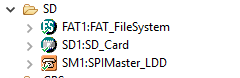
\includegraphics[width=0.5\textwidth]{sd.PNG}
	\caption{Componentes necesarios para permitir el almacenamiento el la tarjeta microSD.}\label{fig:sd.PNG}
\end{figure}
\FloatBarrier

Hay que relacionar y configurar todos los componentes (como por ejemplo \textit{SPIMaster\_LDD} estableciendo cuales serán los pines de entrada y salida de datos de la placa con el pc).

Para poder trabajar con el acelerómetro es necesario añadir también \textit{FXOS8700CQ} que contiene varias funciones entre las que destacan, FX1\_GetX(), FX1\_GetY() y FX1\_GetZ(). Se encargan de obtener los valores de cada eje en ese preciso momento.
Automáticamente se añadirá el componente \textit{GenericI2C} que implementa un \textit{driver} genérico para el bus de comunicaciones en serie I2C (Inter\-Integrated Circuit), de esta forma funciona tanto para controladores de dispositivos lógicos \textit{LDD} (Logical Device Driver) como para los clásicos que no lo son. En nuestro caso particular nos interesa activar la comunicación LDD I2C y esto obliga a añadir un componente más \textit{I2C\_LDD} que encapsula la interfaz de la comunicación I2C.
\begin{figure}[!h]
	\centering
	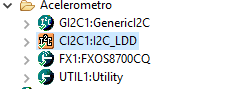
\includegraphics[width=0.5\textwidth]{acelerometro.PNG}
	\caption{Componentes para poder obtener los datos del acelerómetro.}\label{fig:acelerometro.PNG}
\end{figure}
\FloatBarrier

Por último tuve que comprobar que detectaba la tarjeta microSD y que se encontraba montado y funcionando el archivo del sistema (\textit{fileSystemObject}).

\subsection{Mostrar las sentencias NMEA por pantalla}
Para recoger la información del módulo GPS debemos saber que una vez que el módulo conecta con los satélites, produce un \textit{PPS (Pulso por Segundo)} cada 100 milisegundos.
Por lo tanto, lo primero que debemos hacer es añadir los módulos necesarios y configurar los parámetros según el tutorial que me sirvió de guía \cite{tutorial2}. Primero el módulo \textit{ExtInt}, que no es más que una señal externa que se sincroniza con los pulsos del GPS, de forma que así podemos contar los pulsos o simplemente sincronizarlos con otras señales propias.

Segundo, necesitamos AsynchroSerial \textit{AsynchroSerial} una señal asíncrona que implementa el protocolo serie UART y que interactuará con las líneas Rx y Tx del GPS. Como el receptor está constantemente enviando la información con 9600 baudios, debemos seleccionar la misma tasa.
\begin{figure}[!h]
	\centering
	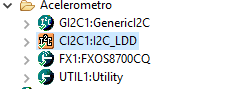
\includegraphics[width=0.5\textwidth]{acelerometro.PNG}
	\caption{Componentes necesarios del módulo GPS.}\label{fig:gps.PNG}
\end{figure}
\FloatBarrier

Ahora con los módulos añadidos y configurados quedaba añadir el código que permitiera la visualización de las sentencias NMEA a través de la terminal Termite. Con esto era suficiente, pero como veremos en el siguiente punto, al añadir \textit{FreeRTOS} se incorpora una cadena de caracteres donde almacenar las sentencia NMEA y un manejador de la misma \textit{(xQueueHandle)}.

\imagen{imprime.PNG}{Función Imprime encargada de pasar los datos al pc por puerto serie.}

\subsection{Almacenar las sentencias NMEA en la tarjeta microSD}
Ahora que ya tenemos la configuración hecha (de las coordenadas del acelerómetro), que permite el almacenamiento de datos en la tarjeta SD, parece obvio que tan solo fuera necesario reutilizar la cadena ya rellenada con nuestra información, pero aquí vino una de las mayores dificultades, se perdía información muy probablemente porque antes de que acabara de escribir en la cadena se empezaba a escribir en la tarjeta microSD y viceversa, de forma que se optó por incluir un sistema operativo en tiempo real como \textit{FreeRTOS}. Para ello tuve que documentarme, añadir dos módulos necesarios al proyecto para que funcionara, \textit{FreeRTOS} y \textit{KinetisSDK}, y crear las tareas pertinentes con su nivel de prioridad asociado. De esta forma, ahora la información que se muestra en la pantalla se pasa directamente a la función \textit{EscribeSD()} encargada de escribir una cadena dada, en la tarjeta microSD.

Como medida de eficiencia se optó por únicamente almacenar los mensajes NMEA de tipo GPRMC, que aportan toda la información que nosotros necesitamos reduciendo en un 75\% la cantidad de datos almacenados.

Los datos se introducen en la cadena con el método \textit{xQueueSendToBack} (dado que es una cola FIFO) y se extraen con \textit{xQueueReceive} por el final de la cola. 
\imagen{chargps.PNG}{Tarea en tiempo real dedicada a recibir e introducir los caracteres en la cadena.}

De manera adicional se decidió dar utilidad al diodo led rgb que incorpora la placa y se configuró de forma que emitiera luz verde (\textit{LEDR\_Off()y LEDG\_Neg()})cuando estuviera recolectando datos del GPS y luz roja(\textit{LEDR\_Neg()y LEDG\_Off()}) cuando estuviera ocupado escribiendo en la tarjeta microSD.
\imagen{escribeSD.PNG}{Código necesario para el correcto envío de datos a la tarjeta microSD.}

\subsection{Añadir un sistema en tiempo real}
En un principio cabe destacar que no incluimos un sistema operativo de tiempo real, lo cual generaba diferentes problemas, el principal es que era necesario programar la gestión y planificación de las tareas, utilizando hilos, interrupciones periódicas etc. Esto cuando el problema es sencillo se puede hacer, pero cuando el problema empieza a complicarse es mejor delegarlo en un RTOS. 

En consecuencia, la información almacenada no correspondía en muchas ocasiones con la mostrada por pantalla. 
Más adelante descubrimos que esto se debía a que muy probablemente estuviéramos almacenando información en nuestra cadena antes si quiera de llegar a escribir por completo la que ya teníamos en el buffer. Utilizamos FreeRTOS por ser uno de los más extendidos para pequeños sistemas embebidos. Añadimos el módulo correspondiente en Kinetis \textit{FreeRTOS} y lo configuramos.
\imagen{tareas.PNG}{Inicialización de tareas de tiempo real.}

\subsection{Elección de la API para representar las rutas}
Puede parecer un tema trivial, pero se le dio bastante importancia. En un primer momento siempre se consideró la opción de utilizar la de Google Maps, de hecho se llegó a realizar el código para que funcionara (y así lo hizo), pero desde junio de 2018 se convirtió en una API de pago, si bien te otorgan en tu cuenta de Google Maps, 300\$ al mes de crédito para gastar en su API en función del tráfico que tengan tus mapas creados, había que introducir una forma de pago por si excedías el límite, por lo que no me pareció la mejor de las opciones.
\begin{figure}[!h]
	\centering
	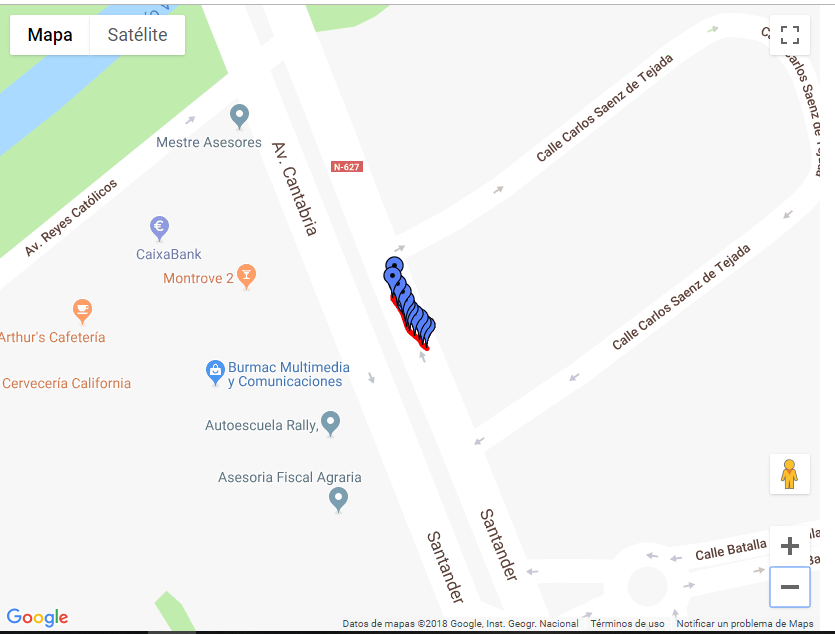
\includegraphics[width=0.7\textwidth]{google.PNG}
	\caption{Mapa creado con la API de Google.}\label{fig:google.PNG}
\end{figure}
\FloatBarrier

De forma que busqué una alternativa gratuita, es ahí donde descubrí Mapbox, una API que poco tiene que envidiar de la de Google. Con un funcionamiento similar multitud de opciones y gratuita. Ya cuenta con numerosas empresas que usan sus servicios como: Tinder, Bosch, National Geographic, Mastercard, CNN o Snapchat entre las más importantes.
\imagen{empresas.PNG}{Empresas que ya trabajan con Mapbox.}

\subsection{Creación de una interfaz básica HTML}
Con la ayuda de la documentación de Mapbox\cite{mapboxapi} se creó una primera página HTML sencilla que mostraba unas coordenadas pasadas directamente en un array. Pensé que tendría que leer las que yo había capturado de forma aislada y pasárselas. Por fortuna descubrí que se podía pasar el fichero entero en formato GeoJSON. Convertí mi archivo NMEA a GeoJSON con una herramienta web y pasándoselo o bien de manera local o un enlace raw de GitHub funcionaba perfectamente. Pero el objetivo era automatizar este proceso y que la mayoría de acciones fueran transparentes al usuario.
\begin{figure}[!h]
	\centering
	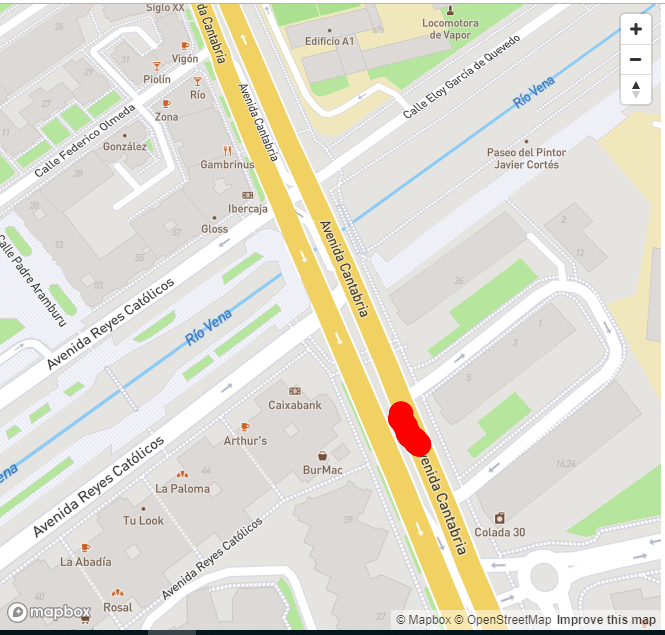
\includegraphics[width=0.7\textwidth]{mapboxgeojson.PNG}
	\caption{Mapa creado con la API de Mapbox.}\label{fig:mapboxgeojson.PNG}
\end{figure}
\FloatBarrier

\subsection{Conversión automática de NMEA a GeoJSON}
Tras mucho investigar descubrí que la conversión de NMEA a GeoJSON es una de las menos frecuentes, son más típicas otras como GPX (para el caso del receptor Garmin) o KML en el caso de querer representar en Google Maps. Estuve barajando hacer un parser manualmente, pero tendría que dedicar muchos recursos en aprender las espeficaciones del estándar GeoJSON, así que por temas de eficiencia opté por buscar un recurso que lo agilizara. Descubrí MyGeodata, que es sin ninguna duda el mejor sitio web para convertir entre cientos de estándares. Solo había un problema y era que de forma gratuita solo ofrece 3 conversiones mensuales, pero tras hablar con el soporte y explicar mi situación de estudiante, me ofrecieron una \textit{key} gratuita. 

Con la ayuda de su documentación,\cite{mygeodataapi} desarrollé el código, pero entre los parámetros que había que poner para poder hacer uso de su herramienta se encontraba uno que me estaba dando problemas. Se trata de \textit{outcrs}, (sistema de referencias de coordenadas de salida) que no sabía qué había que indicar, más allá del formato de salida que se deseaba. Por defecto se realiza mediante \textit{'EPSG:3857'}, necesario para conversiones para la API de Google en KML, en nuestro caso Mapbox necesitaba GeoJSON de forma que nos correspondía \textit{'EPSG:4326'}.
\imagen{outcrs.PNG}{Información básica que necesita para poder convertir el archivo.}

\subsection{Habilitar la subida de archivos al servidor}
La opción más cómoda y amigable que se me ocurrió para el usuario, con la que estuviera familiarizado, fue que realizara la subida del archivo tal cual lo encontraba en la microSD. La parte del \textit{backend} se encargaba de convertirlo y cargarlo, con la opción que brinda en un futuro tener los archivos en el servidor para poder mostrar el mapa deseado por el usuario.
 
La subida se hace mediante un formulario que llama al archivo \textit{upload\_file.php} que es el encargado de casi todo. En un principio se representaba el mapa en la página principal, pero al no tener todavía las coordenadas y estar vacío se decidió mover a una página secundaria con el fin de optimizar la página de inicio.
\imagen{upload.PNG}{Formulario que habilita la subida de archivos.}
\imagen{uploadgrafico.PNG}{Interfaz de subida de archivos familiar para el usuario.}

\subsection{Configuración de XAMPP y Python} 
En el anterior punto para la correcta ejecución del código PHP, instalamos XAMPP en nuestro ordenador para trabajar de manera local y que luego fuera fácilmente exportable a un servidor si así se requiere en un futuro. De manera nativa XAMPP no permite la ejecución de Python, pero se puede conseguir añadiendo la extensión \textit{.py} a la \textit{Common Gateway Interface} (interfaz de entrada común) como se detallará en el manual del programador.
De esta forma utilizo la función \textit{shell\_exec} para que ejecute el script encargado de la conversión de NMEA a GeoJSON.
\imagen{convert.PNG}{Llamada al script que convierte las coordenadas.}

\subsection{Descomprimir el archivo generado por MyGeodata}
La conversión de coordenadas genera un archivo comprimido, por lo tanto, para que pueda tener acceso, debemos primero descomprimirlo. Esto se realiza mediante la creación de una variable de tipo \textit{ZipArchive} de PHP, la cual tiene un método dedicado a la extracción del contenido (\textit{extractTo()}) y lo almacena en otra carpeta.
\begin{figure}[!h]
	\centering
	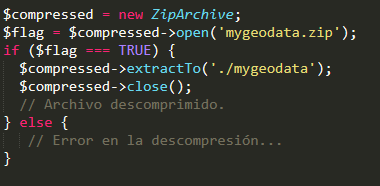
\includegraphics[width=0.7\textwidth]{zip.PNG}
	\caption{Descompresión del \textit{zip} generado por MyGeodata.}\label{fig:zip.PNG}
\end{figure}
\FloatBarrier

\subsection{Añadir fecha y hora a los documentos}
Se planteaba un problema, al subir archivos con el mismo nombre se sobreescribían, para solventarlo se pensó en acompañarlos de la fecha y la hora de forma que cada uno tuviese un nombre único sin tener que forzar al usuarios a renombrarlos ni que se sobresscribieran perdiendo los datos anteriores. Utilizamos la función \textit{date} de PHP y un formato del tipo \textit{dd-mm-yyyy\_h-m-s\_} delante del nombre del fichero.
\imagen{fechas.PNG}{Documentos con el día y la fecha en el título.}

\subsection{Exportar imagen del mapa mostrado y Geolocalización}
Para que el usuario se pueda llevar una instantánea del mapa generado con la ruta, se ha incluido un botón que habilita la descarga de una imagen. Se ha conseguido habilitando el \textit{buffer} de lo dibujado \textit{preserveDrawingBuffer:true} y recuperándolo más tarde cuando demos al botón llamando a \textit{getCanvas()} \cite{descargaimagen}

De igual forma se añadió otro botón para centrar el mapa basándose en tu posición actual. Para ello, se requiere el permiso por parte del navegador y en última estancia del usuario, para poder acceder a tu posición.
\imagen{botones.PNG}{Código que habilita los botones de control, la descarga del mapa y el centrarlo en tu posición.}

\subsection{Añadir una plantilla HTML}
Una vez que la aplicación era funcional, era hora de dotarla de una interfaz agradable al usuario, se utilizó una plantilla basada en \textit{Bootstrap} \cite{plantilla} para la página de inicio, que tras una serie de cambios como: imagen de fondo, textos, imágenes y crear los botones de subida de los archivos, quedó finalizada. Cabe destacar que botones como: ``Iniciar sesión'', ``About'', ``Contact'', ``Terms of Use'', ``Privacy Policy'', los de las redes sociales o el formulario del \textit{email} no se han implementado, pero se han dejado por estética y como línea de mejora de futuro. La página a la que da acceso tras la subida de los ficheros carece de plantilla pues se muestra el mapa a lo largo de la pantalla y contiene 3 botones.
\imagen{pagina.PNG}{Página de inicio con los botones de subida del archivo.}

\subsection{Despliegue de la aplicación}
Para que se pudiera probar la herramienta se necesitaba una placa de desarrollo correctamente programada, o una ruta previamente registrada y una página web. Pensamos que \textit{hostear} la página sería una buena opción, sin embargo finalmente no fue la medida adoptada por diversos motivos. En dominios como \textit{x10hosting} , \textit{5gbfree}, \textit{000webhost} que presentaban una buena oferta gratuita de navegación y número de páginas máximas alojadas, tenían la limitación de no ofrecer Python de forma gratuita, con lo cual no se podía ejecutar la conversión. También se probó en ``GitHub Pages'' arrojando el mensaje ``405 not allowed'' al tratar de ejecutar el código en Python y finalmente tampoco fue posible en \textit{OpenShift} ni \textit{Heroku}. 

Optamos por realizar nuestro despliegue sobre una máquina virtual de Windows 7 limpia que se incluirá en la entrega. Se instaló XAMPP y Python y se configuró correctamente para el correcto funcionamiento.

\subsection{Activación/desactivación por acelerómetro}
Más adelante retomamos una actividad pendiente, que el registro de los datos en la tarjeta microSD dependiera del movimiento con el fin de no almacenar coordenadas de forma repetitiva, por ejemplo en un semáforo. Lo primero fue calibrar el acelerómetro, suponiendo una fuerza de 0G en los ejes 'x' e 'y' y 1G en el eje 'z' proveniente de la gravedad de la tierra, mediante los métodos \textit{FX1\_CalibrateX1g()}, \textit{FX1\_CalibrateY1g()} y \textit{FX1\_CalibrateZ1g()} respectivamente. Más tarde, pusimos como condición que si no se sobrepasaba una fuerza, que establecimos como la mínima para evitar errores producidos por microvibraciones, no se escribiera en la tarjeta microSD.
\imagen{codigoacelerometro.PNG}{Código encargado que calibrar el acelerómetro y capturar los valores de los ejes.}

\subsection{Excepciones PHP}
Por último decidimos crear excepciones para tratar de capturar cualquier error que pudiera surgir en la interfaz. Comprobamos que solo se pudieran subir archivos con extensión txt, que son los que genera la placa, que se moviera a la carpeta ``subidas'' correctamente, que contuviera mensajes NMEA en su interior y que el archivo se convirtiese a GeoJSON sin errores.
\imagen{excepciones.PNG}{Excepción en PHP que comprueba que el archivo subido sea de texto.}

\subsection{Problemas encontrados en el desarrollo}
En este apartado explicaremos algunas cuestiones que nos han provocado retrasos y que detallaremos a continuación por si pudiera servir de ayuda en un futuro.

\subsubsection{La placa deja de funcionar}
En algunas ocasiones es probable que la placa deje de funcionar en el modo de \textit{debugueo} OpenSDA y solo se encienda la luz naranja de corriente. Para solventar esto es necesario enchufar la placa al ordenador mientras se aprieta el botón de \textit{reset} de forma que podamos acceder al \textit{bootloader} y allí pegar el archivo OpenSDA\_V2.bin que se proporciona con el proyecto.

\subsubsection{Comunicación del módulo GPS con la placa}
El módulo GPS tiene un interruptor, para que el envío de datos se produzca de forma satisfactoria debe estar posicionado en ``Soft Serial'' y no en la posición ``Direct''.

\subsubsection{Kinetis no ejecuta los cambios que hemos hecho}
En ciertos momentos nos hemos encontrado con que Kinetis no acometía los cambios que se le había hecho al proyecto, para este problema no hemos encontrado una solución al respecto y la única ha sido reiniciar el programa.

\subsubsection{Cómo copiar y pegar proyectos en Kinetis}
Para poder hacer una copia de tu proyecto y así poder hacer modificaciones sin alterar el original debes hacer antes unos pasos previos:
\begin{itemize}
\tightlist
\item
	Al crear el proyecto evita la opción de que haya archivos enlazados y creálo \textit{standalone} para que los proyectos no compartan archivos y sean independientes.
\item
	Dentro de Project>Properties>C/C++ Build>Settings>Build Artifact>Artifact name asegúrate de poner \${ProjectName} de forma que no referencie al nombre del primer proyecto cuando vaya a ser copiado.
\item
	Evita rutas absolutas dentro de Project>Properties>C/C++ Build> Settings>Tool Settings>Include paths y usa relativas.
\item
	Es una buena idea deshacernos de todo el residuo que pueda haber dejado el proyecto padre, para ello Project>Clean
\end{itemize}
Guía extraída de: \href{https://mcuoneclipse.com/2017/02/18/tips-for-making-copy-of-eclipse-cdt-projects-easier/#more-20572}{\texttt{https://mcuoneclipse.com/2017/02/18/tips-for-making...}}

\subsubsection{Aumentar velocidad de compilación}
Es común que tengas que compilar cada poco tiempo, con el objetivo de reducir el tiempo de espera, es buena idea activar la construcción de código de forma paralela, para ello ve a Project>Properties>C/C++Build>Behavior>Enable Parallel Build y selecciona el máximo que permita tu ordenador.